\documentclass[14pt,a4paper]{scrartcl}
\usepackage[utf8]{inputenc}
\usepackage[english,russian]{babel}
\usepackage{misccorr,color,ragged2e,amsfonts,amsthm,graphicx,systeme,amsmath,mdframed,lipsum}
\renewcommand\qedsymbol{$\blacksquare$}
\usepackage[normalem]{ulem}
\renewcommand*{\proofname}{\text{Доведення}}
\theoremstyle{definition}
\newtheorem{defo}{Означення}[section]
\newtheorem*{teo}{Теорема}
\newtheorem*{example}{Приклад}
\theoremstyle{remark}
\newtheorem*{remark}{Зауваження}
\theoremstyle{definition}
\newtheorem*{consequence}{Наслідок}
\theoremstyle{definition}
\newtheorem{statement}{Утверждение}[section]
\newmdtheoremenv{boxteo}{Теорема}[section]
\setlength\parindent{0pt}
\begin{document}
\begin{center}
  КА-96 Терещенко Д.\\
  РР\#3 Вариант - 26
\end{center}
\textbf{1.26}
$y = \displaystyle\frac{e^{  \frac{1}{x} }}{x^2} \quad y=0 \quad x=2 \quad x=1$\\
\begin{figure}[h]
\centering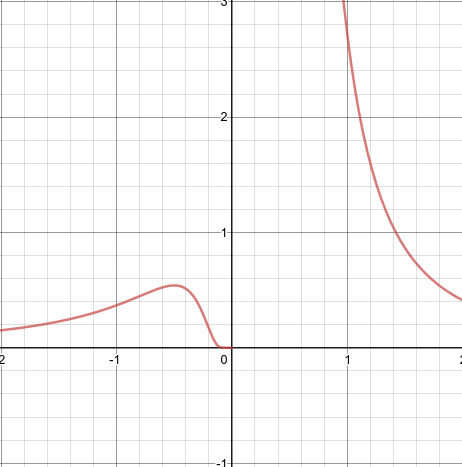
\includegraphics[scale=0.5]{g1}
\caption{$y = \displaystyle\frac{e^{  \frac{1}{x} }}{x^2}$}
\end{figure}
$$ S = \int\limits_{1}^{2}{\frac{e^{  \frac{1}{x} }}{x^2}}dx = \left| \begin{gathered}
 t = \frac{1}{x}\\
 dt = - \frac{1}{x^2}\\
\end{gathered} \quad \begin{gathered}
 t(2) = \frac{1}{2}  \\
 t(1) = 1\\
\end{gathered} \right|  =
 \int\limits_{ \frac{1}{2} }^{ 1}{e^tdt} =
 e^t \Big|^{1}_{\frac{1}{2}} = e - \sqrt{e}
$$
\pagebreak\\
\textbf{2.26} Параметрически заданная функция:\\
$$\left\lbrace \begin{gathered}
x = 3 \cos{(t)};\\
y = 8 \sin{(t)};\\
\end{gathered}
\right.
\qquad y = 4 \sqrt{3} \quad (y\geq 4\sqrt{3})
$$
\begin{center}
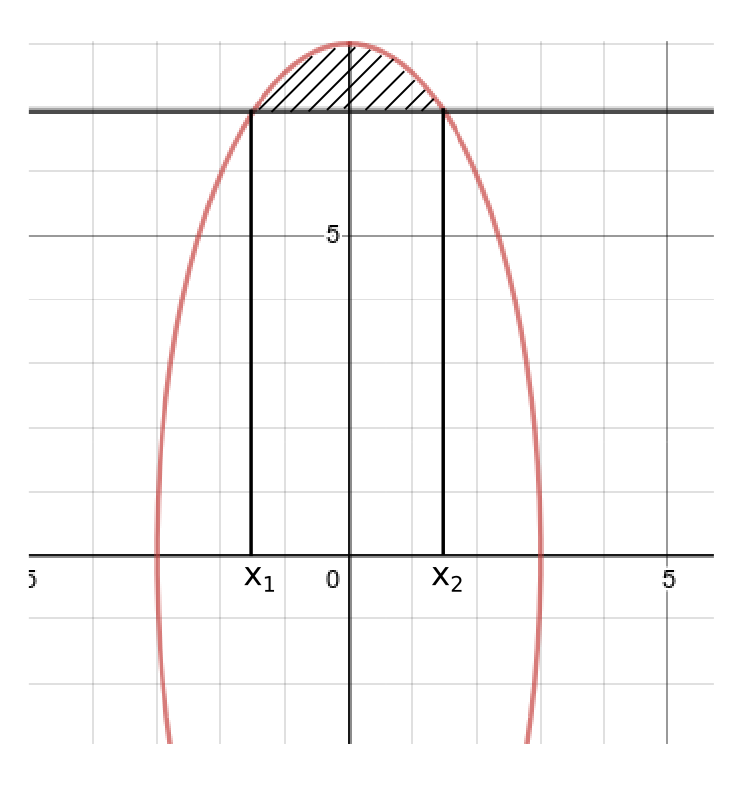
\includegraphics[scale=0.5]{g2.png}
\end{center}

$$
S_{ \varphi} = S_{y} - 4\sqrt{3}(x_2 - x_1) =
\left| \begin{gathered}
x_1 = x(t_1); x_2 = x(t_2)\\
t_2 = \frac{\pi}{3}; t_1 = \frac{2\pi}{3}\\
x_2 = 1,5; x_1 = -1,5
\end{gathered} \right|       = S_y - 12\sqrt{3}
$$
$$S_y  =  \int\limits_{x_1}^{x_2}{y(x)dx} =  \int\limits_{t_1}^{t_2}{y(t)x'(t)dt} =
 -24\int\limits_{ \frac{2\pi}{3} }^{ \frac{\pi}{3} }{\sin^2{(t)}dt } =
12  \int\limits_{ \frac{\pi}{3} }^{ \frac{2pi}{3} }{ 1 - \cos{(2t)} dt}
 $$
 $$
 S_y = \left( t - \frac{\sin^2{(2t)} }{2}  \right)\Big|_{ \frac{\pi}{3} }^{ \frac{2\pi}{3} } = 4\pi + 6\sqrt{3}
 $$
$$
\Rightarrow S_{\varphi} = S_y - 12\sqrt{3} = \mathbf{4\pi - 6\sqrt{3}}
$$
\textbf{3.26}
$$r = 2 \sin{(4\varphi)} \quad \varphi\in [0; \frac{\pi}{4} ] $$
\begin{center}
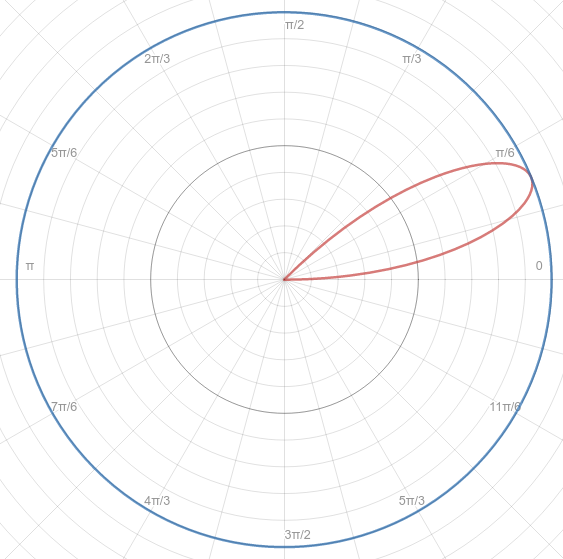
\includegraphics[scale=0.5]{g3.png}
\end{center}
$$
S_{\varphi} = \frac{1}{2}  \int\limits_{0}^{  \frac{\pi}{4} }{4 \sin^2{(4 \varphi)}d \varphi } =  \int\limits_{0}^{ \frac{\pi}{2} }{1 - \cos{(8\varphi)}d \varphi }
$$
$$
S_{\varphi} = \left( 1 -  \frac{\sin{(8 \varphi)}}{8}   \right)\Bigg|_{0}^{ \frac{\pi}{4} } = \mathbf{ \frac{\pi}{4} }
$$
\textbf{4.26}
$$
y = e^x + 26 \quad \ln{\sqrt{8}} \leq x \leq \ln{\sqrt{24}}
$$
График $y(x)$ - экспонента, ''поднятая'' на 26 едениц вверх.\\
Так как мы ищем длинну дуги графика функции, стандартные геометрические превращения не влияют на результат. Поэтому $l_y$ - длинна дуги заданной функции будет: $l_y$ = $l_{e^x}$.
Таким образом, получим: $$
l_y =  \int\limits_{\ln{\sqrt{8}}}^{\ln{\sqrt{24}}}{ \sqrt{1 + (y'(x))^2}dx} = \int\limits_{\ln{\sqrt{8}}}^{\ln{\sqrt{24}}}{ \sqrt{1 + e^{2x}}dx} = \left| \begin{gathered}
 1 + e^{2x} = t^2\\
2x = \ln{(t^2 -1)}\\
dx = \frac{t}{t^2 -1}dt
\end{gathered}
\quad
\begin{gathered}
  t = \sqrt{1+ e^{2x}}\\
  t_1 = \sqrt{9} = 3\\
  t_2 = \sqrt{25} = 5
\end{gathered}
 \right| =
$$
$$
= \int\limits_{3}^{5}{ \frac{t^2}{t^2 - 1} dt} =
 \int\limits_{3}^{5}{1 - \frac{1}{1-t^2}dt }=
 \left( t - \frac{1}{2}\ln{ \left| \frac{1+t}{1-t}  \right| }  \right)\Bigg|_{3}^5 = \mathbf{2 + \ln{ \frac{4}{3} }}
$$
\pagebreak\\
\textbf{5.26}
$$
\left\lbrace \begin{gathered}
 x = 4(2 \cos{(t)} - \cos{(2t)}  )\\
 y = 4(2 \sin{(t)} - \sin{(2t)}  )\\
\end{gathered} \right. \qquad 0 \leq t \leq \pi
$$
\begin{center}
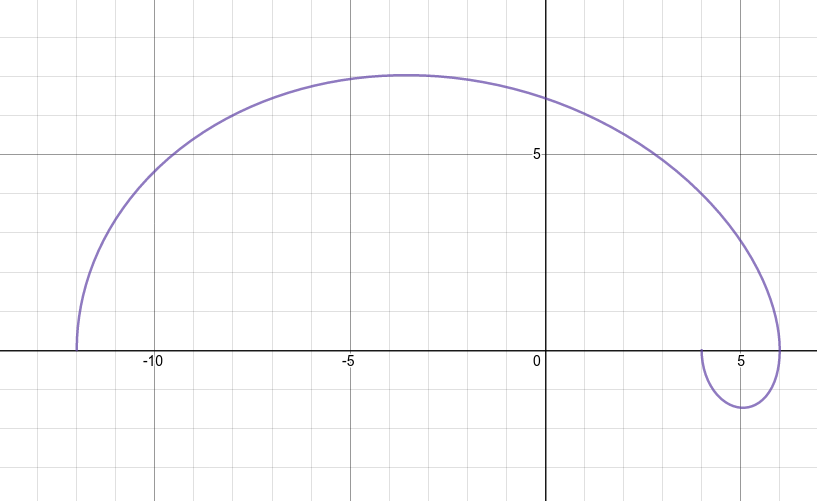
\includegraphics[scale=0.6]{g4.png}
\end{center}
$$
\begin{gathered}
 x'(t) = 8(\sin{(2t)} - \sin{(t)}  )\\
 y'(t) = 8(\cos{(t)} - \cos{(2t)}  )
\end{gathered}
\Longrightarrow (x'(t))^2 + (y'(t))^2 = 64(2 - 2 \cos{t} ) = 256* \sin{\frac{t}{2}}
$$
$$
l_{\varphi} =  \int\limits_{0}^{\pi}{\sqrt{ (x'(t))^2 + (y'(t))^2 }dt} =  16\int\limits_{0}^{\pi}{\sin{ \frac{t}{2} } dt} = \mathbf{32}
$$
\textbf{6.26}
$$
\rho = 2 \cos{\varphi} \qquad 0\leq \varphi \leq \frac{\pi}{6}
$$
$$
l_\rho =  \int\limits_{0}^{ \frac{\pi}{6} }{ \sqrt{ (\rho'(\varphi))^2 + (\rho(\varphi))^2 }d \varphi } =  \int\limits_{0}^{ \frac{\pi}{6} }{ 2\sqrt{ \sin{ (t)}^2 + \cos{(t)}^2   } d \varphi } = 2 \varphi \Big|_{0}^{ \frac{\pi}{6} } = \frac{\pi}{3}
$$
\textbf{7.26}
$$f(x) = x^2 \qquad g(x) = \sqrt{x}$$
Вращение вокруг оси ОХ. Пусть $\exists! x_0 : f(x_0) = g(x_0)$ Значит:\\
$$V =  \pi \left(  \int\limits_{0}^{x_0}{g^2(x)dx} -  \int\limits_{0}^{x_0}{f^2(x)dx} \right) = \pi  \int\limits_{0}^{x_0}{g^2(x) - f^2(x)dx} $$
Соответствующую точку $x_0$ найдём графически или из уравнения $x^2 = \sqrt{x}:$
\begin{center}
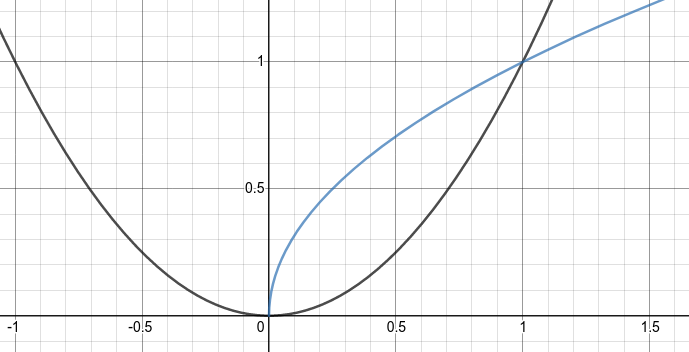
\includegraphics[scale=0.7]{g5.png}
\end{center}
$$x_0 = 1 \Longrightarrow V = \pi \int\limits_{0}^{1}{x - x^4dx} = \pi \left( \frac{x^2}{2} - \frac{x^5}{5} \right)  \Big|_0^1= \mathbf{0.3}\pi $$

\end{document}
